\section{How the same strategy becomes Python and Rust}
\label{sec:implementations}

\subsection{One interface, different levels of coverage}
The Python distribution \path{python/} contains:
\begin{itemize}
 \item binary/quadtree construction, weak/strong/complementary rules and a column-pivoted-QR ID;
 \item exact and proxy compression;
 \item recursive skeletonization, Schur updates, LU/root solve;
 \item a complex one-dimensional interpolative butterfly and DFT/FIO test problems;
 \item ten showcase entries and all twelve problem-oriented experiments, with saved data and figures.
\end{itemize}
The Rust distribution \path{rust/} deliberately has two separate pieces:
\begin{itemize}
 \item a clean main crate: real $f64$ QR compression, apply, storage/timing, direct FFT and exact DFT-butterfly factors;
 \item a separate \path{core-prototype}: trees, admissibility, exact/proxy compression, complex FIO and recursive LU solve with hand-written numerical routines.
\end{itemize}
The Python tree is the more complete experimental package. Rust is an apply benchmark and feasibility implementation, not a feature-complete port of the Python special functions or physics.

\subsection{What each library gives me: reuse, short examples and checked boundaries}
The practical value of the shared choices is visible in the call graph: an application supplies geometry, a kernel and its special sampling/physics rules, while the library executes the generic block work. Table~\ref{tab:reuse-map} names actual shipped routines rather than an aspirational unified API.

\begin{longtable}{@{}>{\raggedright\arraybackslash}p{0.16\textwidth}>{\raggedright\arraybackslash}p{0.25\textwidth}>{\raggedright\arraybackslash}p{0.25\textwidth}>{\raggedright\arraybackslash}p{0.25\textwidth}@{}}
\caption{Abstraction $\to$ shared implementation $\to$ short application file $\to$ checked scope. Paths are relative to \texttt{python/} or \texttt{rust/} as marked.}
\label{tab:reuse-map}\\
\toprule
Abstraction & Shared routine & Short application entry & What is actually checked \\
\midrule
\endfirsthead
\toprule
Abstraction & Shared routine & Short application entry & What is actually checked \\
\midrule
\endhead
Partition & \path{unified.core.Tree} & \path{python: unified/bench/problems.py}, \path{unified/showcase/models.py} & Binary/quadtree boxes over supplied coordinates, including duplicated coordinates for block dofs and two trees for transforms. \\
Admissibility & \path{Weak}, \path{Strong}, \path{Complementary} in \path{unified.core} & One constructor in the Laplace, LS or butterfly setup & Weak/strong recursive solves and complementary butterfly applies; the interaction-geometry experiment compares their storage conventions explicitly. \\
Representation & \path{interp_decomp}, \path{ExactCompressor}, \path{ProxyCompressor} & A kernel closure plus optional proxy override in an experiment file & Column-pivoted-QR IDs, true-far/proxy comparisons and per-box skeletons; non-PDE proxy failure is retained as a result. \\
Recursive assembly & \path{unified.drivers.rskel.rskel_factor} & Laplace example below; Stokes, Yukawa, heat, LS and Matérn setups & Factor/solve against dense references, root sizes, pivots and stored costs where reported. the congruent Helmholtz path is an explicit complex-elimination variant. \\
Butterfly assembly & \path{unified.drivers.butterfly_id} & FIO, DFT and SHT problem definitions & Nested ID factors, apply/transpose apply, DFT exact entry count and ALF per-order measurements. The teacher constructor reads full tiles. \\
Real Rust apply & \path{KernelProblem::benchmark} and \path{HMatrix::from_dense} & \path{rust/examples/laplace.rs} (12 lines), \path{gaussian.rs} and \path{screened.rs} (11 each) & Dense-to-compressed storage, achieved apply error and same-process apply timings. Construction remains a dense oracle. \\
Rust FFT / DFT & \path{rust/src/fft.rs} and \path{examples/dft_as_butterfly.rs} & \path{rust/examples/fft.rs} (38 lines), \path{dft_as_butterfly.rs} (55) & Independent FFT comparison, rank one at every stage and exact $2N\log_2N+2N$ factor storage. \\
Broader Rust core & Separate \path{core-prototype/src/main.rs} & Its case/golden harness, not the main crate's API & Trees, admissibility, proxies, complex FIO and recursive LU; 72 exact golden values, 17 documented QR count differences and separately checked errors. \\
FMM / wideband FMM & Algorithm map and mathematical exposition only in this delivery & No production S2M/M2L/wideband translation example is claimed & The report explains translation and switching; the shipped Python/Rust libraries must not be described as full FMM or wideband implementations. \\
\bottomrule
\end{longtable}

\subsection{A short Python use case}
The entire construction uses an ordinary Laplace test curve. The library owns grouping, compression and solve sweeps; the example supplies no numerical infrastructure.
\begin{lstlisting}[language=Python]
from unified.core import ProxyCompressor, Tree, Weak
from unified.bench import problems as P
from unified.drivers.rskel import rskel_factor
import numpy as np

prob = P.p1_curve(512)
tree = Tree(prob.X, max_leaf=32)
compressor = ProxyCompressor(prob.kernel, prob.X, 1e-8, A=prob.A)
factor = rskel_factor(prob.A, tree, Weak(), compressor)
b = np.ones(512)
x = factor.solve(b)
print(P.relres_kernel(prob, x, b))  # 9.412e-10
\end{lstlisting}
A pivoted QR produces interpolation data used to eliminate redundant interactions. A new kernel replaces the problem and, where necessary, its sampling layer. The reported residual $9.412\times10^{-10}$ is independently computed from the kernel rather than by reusing only the approximate factor. At this size, the measured root has 160 unknowns. This is a recursive-solver example, not a proof that a production FMM is obtained by changing one line.

\subsection{A short Rust use case}
The Rust interface likewise places a kernel closure above common dense construction, compression and measurement code:
\begin{lstlisting}
let problem = KernelProblem::new(
  "log / Laplace", grid(n),
  |x, y| {
    let r = (x - y).abs();
    if r == 0.0 { 1.0 } else { -r.ln() / (2.0 * std::f64::consts::PI) }
  }
);
let result = problem.benchmark(32, 1e-6);
\end{lstlisting}
The full working \path{examples/laplace.rs} has 12 lines. Gaussian and screened-exponential examples each have 11 lines. ``One file per problem'' means a small user-facing file; carefully tested QR, sparse factor and timing machinery remains in the library. The direct FFT and exact DFT-butterfly examples are longer because they also assert structural identities.

\subsection{Problem-specific code is the mathematical contribution}
The showcase metadata separates \textbf{dial code} (kernel adapters, proxy/sampler changes, wrappers and any algebra variant) from \textbf{physics code} (formulation, quadrature, geometry and analytic references). Counts are generated from \path{python/unified/showcase/results.json}; they exclude blank lines, comment-only lines and docstrings. They measure the current named objects, not the intellectual cost of the underlying mathematics.

\begin{longtable}{@{}>{\raggedright\arraybackslash}p{0.19\textwidth}>{\raggedright\arraybackslash}p{0.12\textwidth}>{\raggedright\arraybackslash}p{0.14\textwidth}>{\raggedright\arraybackslash}p{0.43\textwidth}@{}}
\toprule
Showcase problem & Dial lines & Physics lines & Problem-specific structure still supplied \\
\midrule
\endhead
Laplace & 14 & 38 & Double-layer formulation, geometry, source-generated exact solution. \\
DFT & 19 & 8 & Bit-reversal wrapper and exact DFT/FFT reference. \\
FIO & 9 & 8 & Phase/amplitude definition and independent application check. \\
Helmholtz & 76 & 41 & the congruent complex-elimination driver plus oscillatory boundary quadrature/reference. \\
Stokes & 85 & 94 & Block proxy, completed formulation, normals, rigid modes and analytic mobility checks. \\
Yukawa & 32 & 44 & Screened double layer, monopole-column compatibility and exact exterior-source solution. \\
Heat / Rothe & 77 & 66 & Absolute tolerance, screening truncation, history layers and semi-discrete reference. \\
Fractional & 31 & 47 & Lifted proxy geometry plus lattice correction and Getoor reference. \\
Lippmann--Schwinger & 31 & 71 & Two-sided contrast kernel, singular self-cell and Bessel-series reference. \\
Spherical harmonics & 49 & 71 & Table/transpose adapter plus ALF recurrence, Gauss nodes and physical invariants. \\
\bottomrule
\end{longtable}

The sharp contrast is with the original Python core+drivers snapshot used by the reference-port map: 851 physical lines, of which 351 are counted algorithmic code lines. The separate Rust feasibility prototype implements 1104 algorithmic lines plus 513 golden-harness lines. Its size reflects hand-written QR/LU, complex arithmetic and broader cases; it is not folded into the lean main crate. Current packaging changes the reference-loading path, so the historical 851-line figure is quoted specifically for that port-map snapshot.

\subsection{What the measurements show}
At $N=2048$, leaf size 32 and $\eps=10^{-6}$, the saved Rust release sweep gave:
\begin{table}[htbp]
\centering\small
\begin{tabular}{@{}lrrrrr@{}}
\toprule
Problem & Storage / dense & Apply error & Dense (ms) & Compressed (ms) & Speedup \\
\midrule
Log/Laplace & 0.0767 & $2.77\times10^{-7}$ & 0.676 & 0.057 & $11.8\times$ \\
Gaussian covariance & 0.0576 & $2.82\times10^{-7}$ & 0.647 & 0.051 & $12.6\times$ \\
Screened exponential & 0.0361 & $1.04\times10^{-15}$ & 0.661 & 0.045 & $14.7\times$ \\
\bottomrule
\end{tabular}
\caption{Rust compressed-apply measurements in the same release-built process. They are not Rust-versus-Python language ratios.}
\label{tab:rustbench}
\end{table}

\begin{figure}[htbp]
\centering
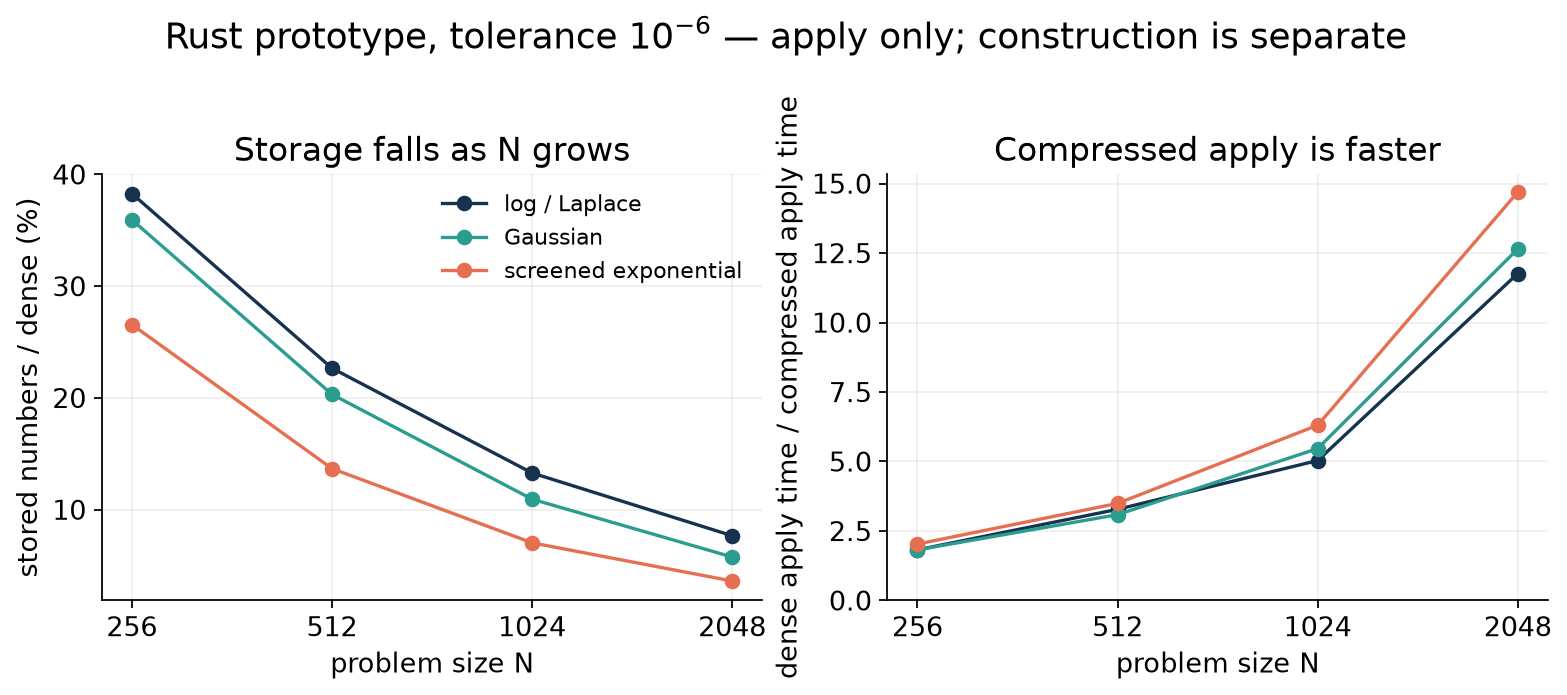
\includegraphics[width=\linewidth]{figures/rust-scaling.png}
\caption{Compressed storage decreases as a fraction of dense, while repeated apply becomes faster. Construction is reported separately.}
\label{fig:rustscaling}
\end{figure}

Compression itself took about $0.96$ seconds per problem at $N=2048$; dividing by the measured saving per call gives an estimated break-even after roughly 1,560, 1,619 and 1,559 applies for log/Laplace, Gaussian and screened exponential respectively. These are \textbf{dense-to-compressed oracle factors}, best suited to repeated apply: construction is not a fast hierarchical builder. Raw samples, min/median values and peak RSS are in \path{rust/results/summary.json}.

The exact DFT-butterfly example at $N=1024$ has $22{,}528=2N\log_2N+2N$ stored entries, every stage rank one and relative error $1.83\times10^{-16}$ against a separate FFT. The main Rust crate has 21 recorded passing checks. The broader core prototype has 72 exact golden values and 17 explicitly documented QR-tolerance-boundary count differences. Its recorded errors remain below $10^{-8}$ and LU residuals are at most $1.724\times10^{-15}$. Parity is judged by achieved accuracy rather than bit-identical rank counts.

For the Python generic B1 butterfly, stored entries/dense at $N=4096,t=1$ are $0.116$ at $\eps=10^{-6}$ and $0.150$ at $\eps=10^{-8}$. These ratios describe that driver and tolerance, not every oscillatory operator.

\subsection{Checked boundaries behind those measurements}
The boundaries are best stated as capabilities and evidence, not as an apology for what is absent:
\begin{itemize}
 \item \textbf{Python:} 126 recorded core tests pass, including all seven restored reference-SVD comparisons; 24 showcase tests pass; 10 spherical-harmonic tests pass after the corrected Gauss-node regression. The collection count of 264 is not an all-long-tests-pass claim.
 \item \textbf{Reference construction:} the Python recursive driver and main Rust dense-to-compressed path retain dense working matrices. They demonstrate achievable factors and solves but do not certify dense-free $O(N\log N)$ construction.
 \item \textbf{Rust coverage:} real scalar apply examples and the separate broader feasibility core are checked. One production-wide Rust API, deliberate production LAPACK selection, the complete physics experiments' special functions, and a matched-backend language-speed comparison are not established.
 \item \textbf{Method coverage:} FMM and wideband FMM are fully explained in the report through their expansion/translation roles; their production operators are not silently attributed to the small reference libraries.
\end{itemize}
Exact provenance and per-suite commands are recorded in these guides:
\begin{itemize}
 \item \path{python/docs/STATUS.md} and \path{python/docs/TESTING.md};
 \item \path{rust/PORT_STATUS.md} and the receipts under \path{results/}.
\end{itemize}

\section{Conclusion: one strategy, many algorithms}
The framework's most useful contribution is not a menu from which any solver follows automatically. It is a common way to \textbf{read, diagnose and test} a hierarchical method:
\begin{enumerate}
 \item Find an interaction matrix's useful groups and orderings.
 \item Decide which interactions a short representation can describe safely.
 \item Derive or choose that representation, with rank/error evidence.
 \item Obtain it through an honest sampling/access model.
 \item Assemble it by the relevant translation, sparse-factor recursion or elimination, and measure build, storage, apply and stability separately.
\end{enumerate}
FMM and wideband FMM make grouped summaries powerful through expansions and scale-specific translations; HBS/RS and FMM-LU turn them into direct solves through elimination and modified-block bookkeeping; butterflies use complementary tilings and nest local bases; the FFT combines exact residue-class rank one with Cooley--Tukey recursion.

The twelve experiments show the essential research motion: a generic choice works until an identifiable hypothesis fails, and the failure points to the new mathematics---not to a universal ``next solver''. Sometimes that mathematics is an adjoint identity, a richer proxy geometry or a two-sided coefficient. Sometimes it is a negative cost result telling us not to make the proposed change. The shared framework organizes the problem and the evidence; the application-specific mathematics still solves it.
